\documentclass[11pt,a4paper]{article}
\usepackage[utf8]{inputenc}
\usepackage[T1]{fontenc}
\usepackage{lmodern}
\IfFileExists{spanish.ldf}{\usepackage[spanish,es-tabla]{babel}}{\usepackage[provide=*,spanish]{babel}}
\usepackage[margin=2.3cm]{geometry}
\usepackage{graphicx,booktabs,tabularx,longtable,amsmath,float}
\usepackage{xcolor,fancyvrb}
\usepackage[hidelinks]{hyperref}
\definecolor{azul}{HTML}{176B9B}
\DefineVerbatimEnvironment{lstlisting}{Verbatim}{fontsize=\footnotesize,frame=single}
\pagestyle{plain}
\setlength{\parskip}{5pt}\setlength{\parindent}{0pt}
\newcommand{\archivo}[1]{\nolinkurl{#1}}
\setlength{\emergencystretch}{3em}
\setcounter{tocdepth}{1}
\newcommand{\figura}[4]{\begin{figure}[H]\centering\includegraphics[width=#2\linewidth]{figures/#1}\caption{#3}\label{#4}\end{figure}}
\begin{document}
\begin{titlepage}
\centering\vspace*{1.7cm}
{\Large Proyecto final de Robótica Móvil\par}\vspace{0.7cm}
{\huge\bfseries Navegación autónoma de un robot diferencial\par}\vspace{0.6cm}
{\Large Control, fusión sensorial, SLAM, localización y misión con Nav2\par}\vspace{1cm}
{\large Daniela Molina\\Tomás Alvarez Jaimes\\Santiago Chacon Guerrero\par}\vspace{0.8cm}
{\large 22 de noviembre de 2026\par}\vfill
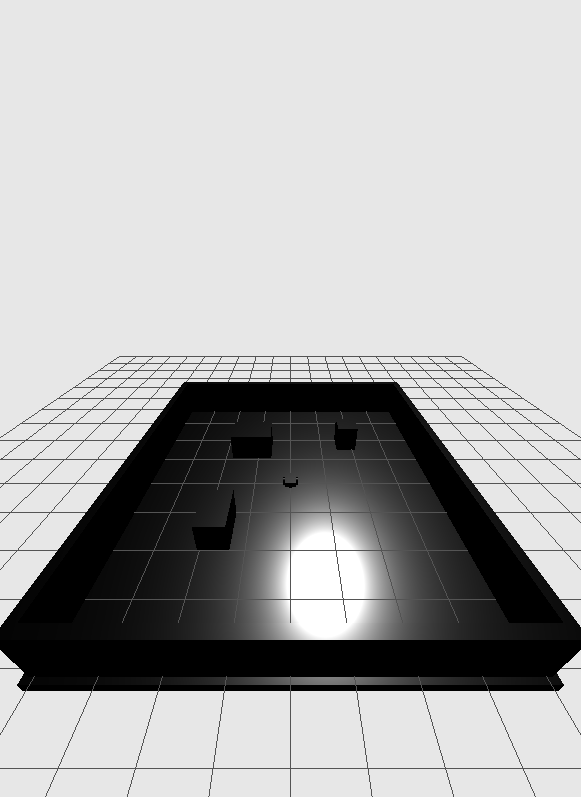
\includegraphics[height=7.5cm]{figures/gazebo.png}\par
{\small Captura propia del entorno simulado \archivo{rbtc_room} en Gazebo Fortress.}\vfill
\url{https://github.com/Daniela6666/proyecto_RBTC}\par
{\small Informe integrado de las prácticas P1--P5 y del proyecto final.}
\end{titlepage}

\begin{abstract}
Se implementó un sistema de navegación autónoma para un robot diferencial propio, usando ROS 2 Humble y Gazebo Fortress en Ubuntu 22.04 sobre WSL2. El trabajo integra control y odometría de ruedas, un filtro de Kalman extendido (EKF), construcción de mapas con SLAM Toolbox, localización probabilística con AMCL y navegación con Nav2. Un nodo de misión lee cuatro objetivos desde YAML y ofrece servicios de inicio y cancelación. Las mediciones documentadas de P1 y P2 muestran que la fusión de la velocidad angular de la IMU reduce el error angular final respecto a la odometría. Los ensayos de P3 y P4 comparan dos velocidades de mapeo y cuatro condiciones de inicialización y ruido del láser. La prueba integrada alcanzó los cuatro objetivos con EKF activo, rechazó un inicio duplicado y ejecutó recuperaciones ante una meta bloqueada. Se presentan los resultados observados, su trazabilidad y las limitaciones de una sola ejecución por condición.
\end{abstract}
\tableofcontents\newpage

\section{Introducción y objetivos}
La navegación autónoma exige relacionar percepción, estimación y control dentro de un sistema de coordenadas coherente. La odometría permite seguir el movimiento local, pero acumula error; el mapa y el láser aportan referencias para corregir la localización global. Nav2 utiliza estas estimaciones para planificar y controlar el movimiento hacia un objetivo.

El objetivo general fue construir y validar una cadena funcional \emph{control $\rightarrow$ EKF $\rightarrow$ SLAM $\rightarrow$ AMCL $\rightarrow$ Nav2}, culminando en una misión iniciada mediante un servicio. Los objetivos específicos fueron comparar las dos alternativas de control, evaluar el aporte de la IMU, construir y guardar un mapa propio, medir la recuperación de AMCL ante una pose incorrecta y ruido del láser, y comprobar la navegación y los servicios de misión.

\section{Plataforma, organización y método}
\subsection{Entorno y robot utilizado}
Se utilizó el paquete propio \archivo{dif_bot}, no un brazo UR5. El URDF describe una base diferencial con dos ruedas motrices, dos apoyos pasivos, LiDAR e IMU. El mundo \archivo{rbtc_room.sdf} contiene una habitación de aproximadamente $8\times8$ m y tres obstáculos. La simulación utiliza Ogre 1 para compatibilidad con el renderizado disponible en WSL.

\begin{table}[H]\centering\caption{Parámetros del sistema revisados en el repositorio.}
\begin{tabularx}{\linewidth}{lX}\toprule
Elemento & Configuración\\\midrule
Sistema & Ubuntu 22.04, WSL2; ROS 2 Humble; Gazebo Fortress\\
Chasis & Caja de $0.40\times0.30\times0.15$ m, frame \archivo{base_link}\\
Ruedas & Radio $0.10$ m; separación $0.38$ m\\
LiDAR & 360 muestras, 10 Hz; alcance máximo 12 m; frame \archivo{laser_frame}\\
IMU & 50 Hz; frame \archivo{imu_link}\\
Mapa & Rejilla de ocupación, resolución $0.05$ m/celda\\
Tiempo & \archivo{use_sim_time:=true}, reloj procedente de Gazebo\\\bottomrule
\end{tabularx}\end{table}

\subsection{Fuentes de evidencia y alcance}
Las cifras de P1 y P2 proceden de la re-medición del robot actual documentada por Persona A en \archivo{docs/informe_A.md}, con fecha 22 de noviembre. Se conserva el PDF de TF del repositorio. Los registros originales de algunas mediciones de A se mencionan en un \emph{scratchpad} no versionado; por ello, este informe los atribuye al documento y no los presenta como una nueva medición independiente.

Los resultados de P3, P4 y P5 proceden de la última tanda aislada de \archivo{scripts/validate_bc.py} y \archivo{scripts/validate_navigation.py}. Se conservan JSON, CSV y mapas PGM. Cada ensayo usa un dominio ROS separado de la sesión de demostración y una partición de Gazebo única para impedir interferencias de procesos de otras corridas. La captura de Gazebo incluida aquí fue tomada al preparar este informe, usando la función de captura del simulador.

Se realizó una ejecución por condición. No se calculan intervalos de confianza ni se extrapola el rendimiento a un robot físico. La prueba de compilación en una copia limpia reutilizó las dependencias del sistema instalado; no equivale a una instalación desde cero de Ubuntu.

\subsection{Estructura funcional y TF}
Durante el mapeo, SLAM Toolbox publica \archivo{map -> odom}; durante la navegación, esa función corresponde a AMCL. El EKF publica \archivo{odom -> base_link}. El publicador del estado del robot relaciona la base con ruedas y sensores. SLAM y AMCL no se ejecutan simultáneamente como autoridades de la misma transformación.

\begin{table}[H]\centering\caption{Entradas y salidas principales de la integración.}
\begin{tabularx}{\linewidth}{lXX}\toprule
Componente & Entradas & Salidas\\\midrule
Control diferencial & Comando de velocidad & Odometría de ruedas, estados articulares\\
EKF & Odometría, velocidad angular IMU & \archivo{/odom_filtered}, TF local\\
SLAM Toolbox & Láser, TF local & Mapa y TF global durante mapeo\\
AMCL & Mapa guardado, láser, TF local & Pose estimada y TF global\\
Nav2 & Pose, mapa, láser, objetivo & Ruta y comandos de movimiento\\
Nodo de misión & YAML, servicios & Objetivos Nav2 y estado JSON\\\bottomrule
\end{tabularx}\end{table}

\section{Práctica 1: control y odometría}
\subsection{Revisión del URDF, sensores y joints}
Se revisaron \archivo{robot.urdf.xacro}, \archivo{gz_control.xacro} y \archivo{ros2_control.xacro}. Los joints \archivo{left_wheel_joint} y \archivo{right_wheel_joint} son continuos, con eje $(0,1,0)$ y centros en $y=\pm0.19$ m. Los joints \archivo{front_joint}, \archivo{rear_joint}, \archivo{laser_joint} e \archivo{imu_joint} son fijos. La base es padre de ruedas, apoyos y sensores. El robot actual no incluye cámara.
\begin{figure}[H]\centering
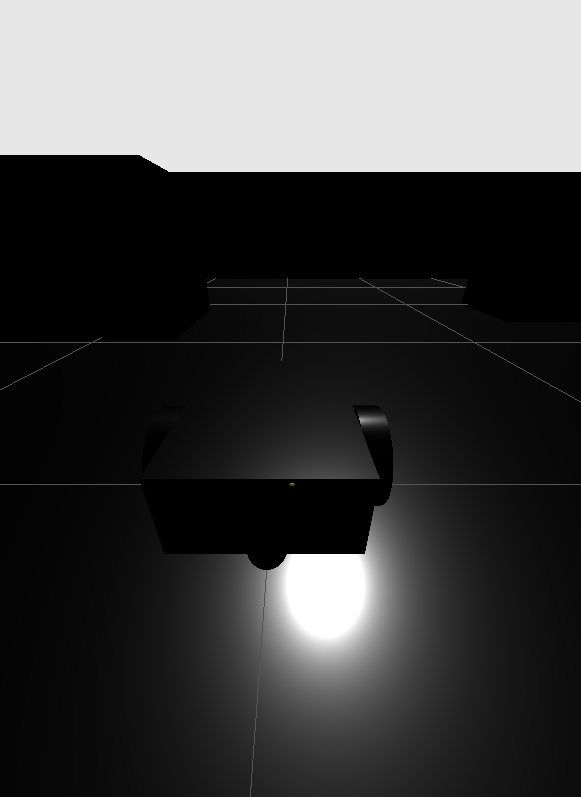
\includegraphics[height=5cm,trim=0 70 0 140,clip]{figures/robot_gazebo.png}
\caption{Segunda captura propia de Gazebo: vista cercana del chasis y las ruedas del robot diferencial. La apariencia oscura corresponde al renderizado observado en la sesión WSL.}
\end{figure}

Para radio $r$ y separación $b$, las velocidades de rueda se relacionan con el movimiento ideal mediante
\begin{equation}
v=\frac{r}{2}(\omega_R+\omega_L),\qquad
\dot\theta=\frac{r}{b}(\omega_R-\omega_L).
\end{equation}
La integración de estas velocidades estima la pose, pero no mide directamente el desplazamiento real del chasis cuando hay deslizamiento u otros errores del modelo.

\subsection{Inciso 1: ¿qué controlador genera la odometría?}
Con \archivo{use_ros2_control:=false}, el plugin nativo \archivo{ignition::gazebo::systems::DiffDrive} calcula la odometría, que el puente expone en \archivo{/odom}. El publicador visible en ROS es \archivo{ros_gz_bridge}. El comando se envía a \archivo{/cmd_vel}.

Con \archivo{use_ros2_control:=true}, el controlador \archivo{diff_drive_controller} calcula y publica \archivo{/diff_drive_controller/odom}. Se activan este controlador y \archivo{joint_state_broadcaster}. En esta configuración el comando se envía a \archivo{/diff_drive_controller/cmd_vel_unstamped}. Ambos modos usan frames \archivo{odom} y \archivo{base_link}, y la misma geometría de ruedas.

\subsection{Inciso 2: estabilidad y latencia}
La tabla recoge las mediciones de Persona A con el robot actual. La frecuencia corresponde al reloj de pared, con una ventana de aproximadamente siete segundos.
\begin{table}[H]\centering\caption{Comparación de control, según la re-medición de P1.}
\begin{tabular}{lrr}\toprule
Magnitud & DiffDrive nativo & ros2\_control\\\midrule
Frecuencia de odometría [Hz] & 29.41 & 49.99\\
Desviación del intervalo de odometría [ms] & 0.11 & 0.14\\
Frecuencia LiDAR [Hz] & 10.00 & 9.99\\
Frecuencia IMU [Hz] & 49.87 & 47.98\\
$x$ real tras avance [m] & 0.9856 & 0.9800\\
$x$ odométrico tras avance [m] & 0.9856 & 0.9800\\
Yaw real tras giro [rad] & 2.6138 & 2.5892\\
Yaw odométrico tras giro [rad] & 2.4660 & 2.4500\\\bottomrule
\end{tabular}\end{table}
El movimiento consistió en avanzar a $0.2$ m/s durante 5 s, detenerse, girar a $0.5$ rad/s durante 5 s y volver a detenerse. Los dos modos mantuvieron roll y pitch aproximadamente nulos en el ensayo documentado. La odometría subestimó el giro real en aproximadamente 5.7\% y 5.4\%, respectivamente. En avance recto coincidió con la referencia física dentro de la resolución indicada. Esto no demuestra igualdad de exactitud en cualquier trayectoria.

La publicación de odometría fue regular en ambos casos. Se observó un hueco de hasta $0.346$ s en la IMU con ros2\_control; la causa no se determinó. La herramienta \archivo{ros2 topic delay} produjo resultados no interpretables por la referencia temporal. La alternativa medida, edad del mensaje respecto a \archivo{/clock}, fue aproximadamente 0 ms para odometría y 1.09--1.19 ms para LiDAR, con resolución de 1 ms y pequeños valores negativos por discretización. \textbf{Estas edades no son una medición de latencia de transporte en tiempo real.} No es válido concluir que un modo tenga menor latencia extremo a extremo a partir de estos datos.

\subsection{Inciso 3: alternativa para un robot real}
Se considera más apropiado ros2\_control para trasladar la solución a hardware, porque separa la interfaz de motores y encoders del controlador diferencial. El plugin nativo de Gazebo resulta conveniente para la simulación rápida. La recomendación es arquitectónica: no se probó hardware físico ni se demostró superioridad de precisión de ros2\_control en estos ensayos.

\section{Práctica 2: fusión sensorial mediante EKF}
\subsection{Inciso 1: sensores y variables fusionadas}
El archivo \archivo{ekf.yaml} configura \archivo{robot_localization} a 30 Hz y en modo bidimensional. Se fusionan $v_x$ y $\dot\theta$ de la odometría, y $\dot\theta$ de la IMU. No se fusionan las posiciones integradas de las ruedas ni la aceleración de la IMU. La selección evita incorporar de nuevo una pose derivada de la misma información de ruedas.

La IMU actual sí aporta orientación en simulación, pero el YAML únicamente habilita velocidad angular. La covarianza de orientación suministrada por el simulador no fue caracterizada; el comentario antiguo que afirma que la IMU no entrega yaw no describe el robot actual. La decisión efectiva se identifica leyendo las máscaras \archivo{odom0_config} e \archivo{imu0_config}.

\subsection{Inciso 2: frame publicado y verificación TF}
Con \archivo{world_frame: odom} y \archivo{publish_tf: true}, el EKF publica \archivo{odom -> base_link}. Para evitar duplicación, se desactiva esa TF en la fuente de odometría: en el modo nativo no se puentea la TF del DiffDrive; en ros2\_control se utiliza \archivo{enable_odom_tf: false}.

La evidencia de Persona A contabilizó 241 mensajes de esta arista en 8 s con IMU, es decir, unos 30.1 Hz. La existencia de varios publicadores registrados en \archivo{/tf} no implica por sí sola una duplicación: se debe comprobar qué arista publica cada uno. En la integración final, AMCL publica \archivo{map -> odom}; se deshabilita la transformación estática provisional de \archivo{ekf.launch.py} con \archivo{launch_static_map_odom:=false}.

\figura{frames_ekf.pdf}{0.95}{Árbol TF obtenido por Persona A con \texttt{view\_frames}, conservado en el repositorio. Corresponde al ensayo del EKF; la arista global provisional se sustituye por AMCL en navegación.}{fig:tf}

\subsection{Inciso 3: efecto de desactivar la IMU}
Se comparó la misma secuencia de avance y giro con IMU habilitada y deshabilitada en el filtro. Deshabilitar su fusión no requiere apagar físicamente el sensor. La referencia fue la pose de Gazebo; no la propia odometría.
\begin{table}[H]\centering\caption{Yaw final documentado en P2, robot actual.}
\begin{tabular}{lrrr}\toprule
Caso & Gazebo [rad] & Odometría [rad] & EKF [rad]\\\midrule
A: nativo + IMU & 2.6623 & 2.5000 & 2.6149\\
B: nativo sin IMU fusionada & 2.6621 & 2.5000 & 2.4990\\
C: ros2\_control + IMU & 2.6621 & 2.5000 & 2.5813\\\bottomrule
\end{tabular}\end{table}
\figura{ekf.pdf}{0.90}{Errores calculados a partir de las poses finales documentadas por Persona A. Cada barra corresponde a un valor final, no a una serie temporal.}{fig:ekf}
En el caso A, el error absoluto bajó de $0.1623$ a $0.0474$ rad, una reducción aproximada del 70.8\%. Sin IMU, el EKF conservó un error de $0.1631$ rad y siguió de cerca a la odometría. En C el error fue $0.0808$ rad; no se determinó por qué la mejora fue menor. La IMU de esta prueba era ideal respecto al giro físico, por lo que el resultado no permite anticipar el comportamiento con sesgo y ruido de un sensor real.

\section{Práctica 3: construcción del mapa con SLAM}
\subsection{Procedimiento}
Se lanzó la simulación con el mundo propio y SLAM Toolbox en modo de mapeo. El sistema recibe \archivo{/scan} y la transformación local del robot. Se recorrió la secuencia $(0,-3)$, $(-3,-3)$, $(-3,3)$, $(3,3)$, $(3,-3)$, $(0,-3)$ y $(0,0)$, en metros. Para repetir las condiciones, el recorrido comparativo se automatizó con realimentación de odometría, en lugar de depender de dos teleoperaciones diferentes. Se limitó la velocidad angular a $0.8$ rad/s y se redujo el avance ante errores de orientación.

Se guardaron los mapas con \archivo{nav2_map_server/map_saver_cli}. El mapa de la corrida lenta se instaló como \archivo{maps/rbtc_room.pgm} y su YAML asociado. AMCL y Nav2 se evaluaron sobre ese mapa, incluyendo sus imperfecciones. El mapeo comparativo utilizó odometría nativa; la prueba integrada de navegación sí utilizó EKF.

\subsection{Inciso 1: resolución del mapa}
La resolución del YAML es $0.05$ m/celda: cada celda representa un cuadrado de 5 cm de lado. La corrida lenta generó $272\times246$ celdas y la rápida $169\times185$. El tamaño de la imagen no es el tamaño físico exacto de la habitación: el SLAM puede extender sus límites por observaciones y artefactos. Ambas imágenes comparten resolución, pero tienen distintos orígenes y extensiones.

\subsection{Inciso 2: errores observados}
\figura{mapas.pdf}{1.0}{Mapas PGM reales obtenidos en la última tanda aislada. Negro: ocupado; blanco: libre; gris: desconocido. El contorno discontinuo indica la región interior usada para evaluar cobertura. Se utiliza la misma escala espacial.}{fig:mapas}
Se observan bordes engrosados, trazos duplicados y regiones reconstruidas fuera del contorno esperado, especialmente en la corrida lenta. La cobertura de espacio conocido no demuestra que ese espacio esté correctamente clasificado. La métrica usada cuenta celdas distintas de desconocido dentro del espacio libre teórico, aun si alguna fue clasificada erróneamente como ocupada.

La distancia geométrica se calculó para celdas ocupadas dentro de $|x|,|y|<3.9$ m respecto a paredes y rectángulos de obstáculos esperados. Es una comprobación aproximada de consistencia, no un error completo de SLAM: no penaliza del mismo modo superficies ausentes, no evalúa los artefactos exteriores y no alinea mapas mediante una optimización posterior.

\subsection{Inciso 3: influencia de la velocidad}
\begin{table}[H]\centering\caption{Resultados de mapeo, una corrida por condición. Ruido LiDAR $\sigma=0.01$ m.}
\begin{tabular}{lrr}\toprule
Magnitud & Lenta & Rápida\\\midrule
Límite lineal [m/s] & 0.20 & 0.50\\
Duración simulada [s] & 165.332 & 83.159\\
Cobertura conocida de región libre [\%] & 99.962 & 100.000\\
Distancia ocupación--geometría: media [m] & 0.0811 & 0.0457\\
Distancia ocupación--geometría: P95 [m] & 0.4950 & 0.1850\\\bottomrule
\end{tabular}\end{table}
En esta tanda, la corrida rápida tardó aproximadamente la mitad y obtuvo menor distancia geométrica que la lenta. Por tanto, \textbf{los datos no respaldan afirmar que la menor velocidad produjo el mejor mapa}. A 10 Hz, el desplazamiento nominal entre barridos es 2 cm a 0.2 m/s y 5 cm a 0.5 m/s cuando se alcanza el límite lineal. Un movimiento mayor entre barridos puede dificultar la asociación, pero el resultado también depende de odometría, giros, cierres de bucle y carga de ejecución. Sin repeticiones ni aislamiento de estos factores, no se atribuye causalmente la diferencia solo a la velocidad. La práctica permite comprobar que un mapa con alta cobertura aún puede contener deformaciones relevantes.

\section{Práctica 4: localización con AMCL}
\subsection{Configuración y método de evaluación}
El lanzamiento de localización carga \archivo{amcl.yaml}, con modelo de movimiento diferencial, modelo láser \archivo{likelihood_field}, 500--2000 partículas, hasta 60 haces y frames \archivo{map}, \archivo{odom} y \archivo{base_link}. Los umbrales de actualización son 0.1 m y 0.1 rad. Se usa el mapa propio guardado.

El bloque AMCL heredado dentro de \archivo{nav2_params.yaml} no determina esta localización: \archivo{localization.launch.py} carga el archivo específico \archivo{amcl.yaml}, mientras \archivo{navigation.launch.py} inicia los servidores de navegación. Esta distinción evita confundir parámetros de ejemplo, como \archivo{base_footprint}, con los activos.

Se probaron inicialización correcta y desplazada $+1$ m en $x$, $+1$ m en $y$ y $+0.6$ rad en yaw, con varianzas iniciales $0.5$, $0.5$ y $0.25$. Para cada pose se utilizaron desviaciones del ruido de rango LiDAR de 0.01 y 0.05 m. El robot giró durante 22 s simulados a 0.3 rad/s y recorrió $(0,-1)$, $(-0.7,-1)$, $(-0.7,0)$ y $(0,0)$.

Se calcularon los errores
\begin{equation}
e_p=\sqrt{(x_{AMCL}-x_{gz})^2+(y_{AMCL}-y_{gz})^2},\qquad
e_\theta=|\operatorname{wrap}(\theta_{AMCL}-\theta_{gz})|.
\end{equation}
La referencia fue la pose física del modelo obtenida de Gazebo. Se declaró convergencia al encontrar cinco muestras consecutivas con $e_p<0.2$ m y $e_\theta<0.15$ rad. El tiempo registrado es el de la primera muestra de esa secuencia, no el de su quinta confirmación. Las medianas de las últimas diez muestras se denominan errores finales.

\subsection{Inciso 1: efecto de una pose inicial incorrecta}
\begin{table}[H]\centering\caption{AMCL: resultados de las cuatro condiciones.}
\begin{tabular}{llrrrr}\toprule
Pose & $\sigma$ [m] & $t_c$ [s] & $e_p$ final [m] & $e_\theta$ final [rad] & P95 $e_p$ [m]\\\midrule
Correcta & 0.01 & 0.070 & 0.0085 & 0.0502 & 0.0696\\
Correcta & 0.05 & 0.030 & 0.0202 & 0.0556 & 0.0590\\
Incorrecta & 0.01 & 4.477 & 0.0323 & 0.0560 & 0.6541\\
Incorrecta & 0.05 & 4.456 & 0.0205 & 0.0755 & 0.7331\\\bottomrule
\end{tabular}\end{table}
Las poses incorrectas iniciaron con un error de posición cercano a $\sqrt{2}$ m y convergieron al criterio definido después de unos 4.5 s simulados. El movimiento aportó observaciones para reducir la ambigüedad. En las inicializaciones correctas el criterio se satisfizo desde las primeras muestras; sus pequeños tiempos no deben interpretarse como una comparación precisa de rapidez del filtro.

\figura{amcl.pdf}{0.98}{Errores calculados desde los CSV de AMCL, respecto a la última pose física recibida de Gazebo. Las líneas discontinuas horizontales señalan los umbrales del criterio de convergencia.}{fig:amcl}

\subsection{Inciso 2: influencia del ruido del láser}
Con inicialización correcta, aumentar $\sigma$ de 0.01 a 0.05 m elevó el error final de posición de 8.5 a 20.2 mm. Con inicialización incorrecta, el error final de posición fue menor en la corrida de mayor ruido, pero aumentaron el P95 de posición y el error angular final. No hubo una degradación monótona en todas las métricas, y los tiempos de convergencia fueron similares.

El ruido cambia la coherencia entre barridos y mapa; su efecto depende del muestreo de partículas y de la trayectoria. Se mantuvo el mismo mapa y no se ajustó un modelo probabilístico nuevo para cada nivel de ruido. Estas cuatro corridas demuestran recuperación para el desplazamiento probado, no garantía de recuperación desde cualquier pose. La comparación utiliza la referencia más reciente sin interpolación temporal, lo que limita la interpretación de errores pequeños durante movimiento.

\section{Práctica 5: navegación con Nav2}
\subsection{Inciso 1: planificador y controlador utilizados}
El planificador configurado en este proyecto es \archivo{nav2_navfn_planner/NavfnPlanner}, con \archivo{use_astar: false}; por tanto, usa expansión de Dijkstra. Esta es la configuración por defecto del proyecto evaluado, no una afirmación sobre todas las versiones de Nav2. NavFn es un planificador global sobre el costmap \cite{navfn}.

El controlador local final es DWB, envuelto por \archivo{nav2_rotation_shim_controller::RotationShimController}. Este componente realiza una alineación inicial cuando el robot difiere suficientemente de la orientación de la ruta. Se incorporó tras observar oscilaciones al solicitar una meta detrás del robot. El umbral angular es 0.5 rad y la velocidad de alineación 0.5 rad/s. La prueba final alcanzó la meta $(-0.85,0)$ m, situada detrás de la pose inicial.

\begin{table}[H]\centering\caption{Parámetros principales de navegación.}
\begin{tabular}{lr}\toprule
Parámetro & Valor\\\midrule
Velocidad lineal máxima & 0.18 m/s\\
Velocidad angular máxima & 0.50 rad/s\\
Radio circular de robot & 0.30 m\\
Radio de inflación & 0.45 m\\
Tolerancia de posición & 0.15 m\\
Tolerancia angular & 0.20 rad\\
Desplazamiento mínimo de progreso & 0.10 m\\
Ventana de progreso & 60 s\\\bottomrule
\end{tabular}\end{table}
Los costmaps utilizan el mapa y las observaciones de \archivo{/scan}. La tolerancia de posición de DWB se igualó con la del verificador de meta para evitar criterios de llegada inconsistentes. El uso del EKF en TF no implica que todos los consumidores de velocidad cambien de topic: la configuración conserva referencias a \archivo{/odom} para componentes de Nav2.

\subsection{Inciso 2: comportamientos de recuperación}
Se utilizó el árbol instalado \archivo{navigate_to_pose_w_replanning_and_recovery.xml}. Incluye replanteo de ruta, limpieza de costmaps y comportamientos de giro, espera y retroceso. La configuración contempla giro de 1.57 rad, espera de 5 s y retroceso de 0.30 m a 0.05 m/s.

Para provocar un fallo se solicitó una meta dentro del obstáculo \archivo{box_c}, en $(1.8,-1.8)$ m. El registro de comportamiento contiene cuatro eventos: giro, espera, retroceso y un nuevo giro. La acción terminó con estado 6, \emph{aborted}; no se presenta como una llegada exitosa. El registro prueba el inicio de esos comportamientos, no que cada recuperación completara íntegramente la distancia o el ángulo configurado. El archivo \archivo{recovery_events.log} se incluye con los datos.

Las metas desde RViz utilizan la acción \archivo{NavigateToPose}. La validación cuantitativa de la meta individual invocó esa misma acción por programa y obtuvo estado 4, \emph{succeeded}. Así se evita confundir la configuración o visualización de RViz con una medición automática de llegada.

\section{Proyecto final: nodo de misión e integración}
\subsection{Diseño del nodo y servicios}
El nodo Python \archivo{mission_node.py} utiliza \archivo{nav2_simple_commander}. Al iniciar una misión lee \archivo{waypoints.yaml}, valida el frame \archivo{map} y comprueba que las coordenadas sean numéricas y finitas. Envía los objetivos secuencialmente y publica un estado JSON en \archivo{/mission/status}, con durabilidad \emph{transient local} para conservar el último estado.

\begin{table}[H]\centering\caption{Interfaz de misión.}
\begin{tabularx}{\linewidth}{lX}\toprule
Interfaz & Función\\\midrule
\archivo{/mission/start} & Servicio Trigger: acepta un inicio si no existe una misión activa. Su respuesta no indica que la misión ya terminó.\\
\archivo{/mission/cancel} & Servicio Trigger: solicita la cancelación de la misión.\\
\archivo{/mission/status} & Mensaje String con JSON: espera de Nav2, navegación, objetivo alcanzado, éxito, cancelación o fallo.\\\bottomrule
\end{tabularx}\end{table}
El trabajador de navegación se separa del ejecutor de servicios para que estos sigan respondiendo. Se corrigió un conflicto de ejecutores durante el desarrollo. El tiempo máximo por objetivo es 300 s de reloj real, mientras que la cinemática de los ensayos se evalúa en tiempo simulado; ambos relojes cumplen funciones distintas.

\subsection{Waypoints y ejecución}
\begin{table}[H]\centering\caption{Objetivos leídos desde YAML.}
\begin{tabular}{rlrrr}\toprule
Orden & Nombre & $x$ [m] & $y$ [m] & yaw [rad]\\\midrule
1 & sur & 0.0 & -0.7 & -1.5708\\
2 & suroeste & -0.7 & -0.7 & 3.14159\\
3 & oeste & -0.7 & 0.0 & 1.5708\\
4 & origen & 0.0 & 0.0 & 0.0\\\bottomrule
\end{tabular}\end{table}
\figura{waypoints.pdf}{0.65}{Esquema de los objetivos configurados. La línea une objetivos para mostrar su orden; no representa una trayectoria medida ni necesariamente la ruta exacta calculada por Nav2.}{fig:waypoints}

El lanzamiento \archivo{bringup.launch.py} incluye simulación, EKF, servidor del mapa, AMCL, Nav2 y nodo de misión. El EKF está habilitado por defecto y no se publica una TF estática global adicional. Debe establecerse la pose inicial de AMCL antes de solicitar la misión. No se debe lanzar otra simulación sobre la misma sesión activa.

\subsection{Validación final}
\begin{table}[H]\centering\caption{Comprobaciones registradas en la última ejecución integrada.}
\begin{tabularx}{\linewidth}{lX}\toprule
Prueba & Resultado observado\\\midrule
Nodos de navegación y AMCL & Estados lifecycle activos antes de las pruebas\\
Meta individual $(-0.85,0)$ & Acción finalizada con estado 4: éxito\\
Meta dentro de obstáculo & Estado 6: abortada; cuatro eventos de recuperación\\
Inicio de misión & Solicitud aceptada\\
Segundo inicio simultáneo & Solicitud rechazada\\
Cancelación & Aceptada; estado \archivo{canceled} registrado\\
Misión posterior completa & \archivo{succeeded}, \archivo{completed=4}\\
Fusión local & EKF habilitado durante la integración\\\bottomrule
\end{tabularx}\end{table}
El archivo \archivo{mission_states.json} registra los cuatro estados de objetivo alcanzado y la finalización. En esta tanda la cancelación ocurrió durante la espera de Nav2; las pruebas de desarrollo descritas en el repositorio también documentan cancelación durante navegación. El éxito de cuatro metas cercanas al centro acredita la misión configurada, pero no una cobertura exhaustiva del mundo ni robustez ante obstáculos dinámicos.

\section{Discusión, limitaciones y conclusiones}
La integración depende tanto de la estimación como de la consistencia de interfaces: frames, nombres de topics, reloj de simulación y propiedad de cada TF. Se evitó mezclar ROS Humble e Iron mediante \archivo{scripts/humble.sh}. También se aislaron las ejecuciones de Gazebo después de detectar que procesos remanentes podían interferir con una partición compartida. Solo se incluyen los resultados de la última tanda aislada de B/C.

La odometría lineal fue cercana a la referencia física en la prueba documentada, pero el giro presentó un sesgo. La IMU aportó información útil para reducirlo mediante el EKF; al deshabilitarla se perdió esa corrección. Los resultados justifican la fusión en el escenario probado, sin demostrar calibración ni desempeño en hardware real.

El mapa permitió localizar y navegar, aunque contiene artefactos. La corrida rápida resultó mejor que la lenta según las métricas empleadas; esto refuerza la necesidad de evaluar los mapas obtenidos y repetir ensayos antes de generalizar una recomendación de velocidad. La cobertura casi completa no debe confundirse con fidelidad geométrica.

AMCL recuperó la pose ante el desplazamiento inicial ensayado y ambos niveles de ruido. El efecto del ruido no fue uniforme en las métricas finales. Se requieren múltiples semillas, más trayectorias y sincronización temporal de referencia para cuantificar robustez y errores pequeños con mayor rigor.

La navegación integrada completó una misión de cuatro objetivos con EKF activo. El rechazo de solicitudes simultáneas y la cancelación proporcionan control explícito sobre la ejecución. Ante una meta imposible se observaron recuperaciones y finalización abortada, comportamiento coherente con no alcanzar un objetivo dentro de un obstáculo.

Como trabajo futuro se propone repetir los ensayos, depurar el mapa, caracterizar covarianzas y sesgos de IMU, probar obstáculos dinámicos y realizar una instalación en un sistema operativo limpio. La validación del repositorio en una copia limpia fue satisfactoria, pero usó dependencias ya instaladas y corresponde al commit registrado en \archivo{clean_build.json}. El video demostrativo es un entregable independiente de este informe.

\appendix
\section{Guía de reproducción}
Desde una terminal Ubuntu con las dependencias del README instaladas:
\begin{lstlisting}
git clone https://github.com/Daniela6666/proyecto_RBTC.git
cd proyecto_RBTC
./scripts/humble.sh colcon build --symlink-install
./scripts/humble.sh ros2 launch dif_bot bringup.launch.py
\end{lstlisting}
En una segunda terminal, con el mismo dominio ROS y entorno:
\begin{lstlisting}
./scripts/humble.sh ros2 run rviz2 rviz2 \
  -d src/dif_bot/config/rbtc.rviz
# En RViz: Fixed Frame = map; establecer 2D Pose Estimate.
./scripts/humble.sh ros2 service call /mission/start \
  std_srvs/srv/Trigger '{}'
./scripts/humble.sh ros2 topic echo /mission/status \
  --qos-durability transient_local
# Cancelacion cuando corresponda:
./scripts/humble.sh ros2 service call /mission/cancel \
  std_srvs/srv/Trigger '{}'
\end{lstlisting}
Para mapeo, en una sesión distinta y sin AMCL simultáneo:
\begin{lstlisting}
./scripts/humble.sh ros2 launch dif_bot sim.launch.py
./scripts/humble.sh ros2 launch dif_bot slam.launch.py
./scripts/humble.sh ros2 run teleop_twist_keyboard \
  teleop_twist_keyboard
./scripts/humble.sh ros2 run nav2_map_server map_saver_cli \
  -f src/dif_bot/maps/rbtc_room --ros-args -p use_sim_time:=true
\end{lstlisting}
Los comandos de las líneas que permanecen ejecutándose requieren terminales separadas. Para repetir los ensayos automatizados, usar los casos de \archivo{validate_bc.py} y después \archivo{validate_navigation.py}; recompilar tras reemplazar el mapa lento para que la instalación contenga el mapa actualizado. Estos ensayos inician su propia simulación.

\section{Cobertura de incisos y trazabilidad}
\begin{longtable}{p{0.15\linewidth}p{0.34\linewidth}p{0.42\linewidth}}
\toprule Inciso & Contenido resuelto & Evidencia principal\\\midrule\endhead
P1.1 & Fuente de odometría en ambos modos & \archivo{informe_A.md}, URDF y controladores\\
P1.2 & Estabilidad y límites de medición de latencia & Tablas P1 del documento de A\\
P1.3 & Selección para hardware real & Arquitectura y análisis de interfaces\\
P2.1 & Sensores y variables fusionadas & \archivo{configuracion/ekf.yaml}\\
P2.2 & TF del EKF y ausencia de duplicación & \archivo{figures/frames_ekf.pdf}, launch\\
P2.3 & Prueba con/sin IMU & P2 de A y gráfica de errores finales\\
P3.1 & Resolución del mapa & YAML de ambos mapas: 0.05 m/celda\\
P3.2 & Errores del mapa & PGM y métricas en \archivo{data/mapping_*.json}\\
P3.3 & Efecto de velocidad & Corridas 0.2/0.5 m/s y mapas comparados\\
P4.1 & Pose inicial incorrecta & \archivo{data/amcl_wrong_*.csv}, JSON\\
P4.2 & Ruido del láser & Cuatro CSV, parámetros y tabla AMCL\\
P5.1 & Planificador y control local & \archivo{configuracion/nav2_params.yaml}\\
P5.2 & Recuperaciones & \archivo{data/recovery_events.log}\\
Final & Servicios y misión de cuatro metas & \archivo{data/navigation.json}, \archivo{data/mission_states.json}\\
Reproducción & Compilación y pruebas unitarias & \archivo{data/clean_build.json} y log\\\bottomrule
\end{longtable}
Los datos de A provienen de su informe del robot actual; no se reutilizan cifras de su modelo anterior. Las notas iniciales de B/C fueron complementadas con los registros posteriores de validación. La configuración incluida en el ZIP conserva el estado local evaluado al redactar este documento, incluidos los ajustes posteriores a la primera integración del repositorio.

\begin{thebibliography}{9}
\bibitem{repo} Equipo del proyecto. \emph{proyecto\_RBTC: código, configuraciones, informes por práctica y validación}. \url{https://github.com/Daniela6666/proyecto_RBTC}. Evidencia local revisada el 22 de noviembre de 2026.
\bibitem{slam} S. Macenski y colaboradores. \emph{SLAM Toolbox: herramientas de mapeo y localización 2D}. \url{https://github.com/SteveMacenski/slam_toolbox}.
\bibitem{navfn} Proyecto Nav2. \emph{Navfn Planner, documentación API de Humble}. \url{https://api.nav2.org/nav2-humble/html/md_nav2_navfn_planner_README.html}.
\bibitem{amcl} Proyecto Nav2. \emph{AMCL, guía de configuración}. \url{https://docs.nav2.org/jazzy/configuration_and_development/configuration_guide/others/configuring_amcl/}. Referencia conceptual; los valores utilizados son los YAML del proyecto Humble.
\end{thebibliography}
\end{document}
